% !TeX spellcheck = en_GB
A common issue with data are outliers or anomalies.
These are observations that do not seem to follow the same pattern as the remaining observations.
This is often due to measurement errors, but it could also be due to a more complex relationship between (potentially hidden) features, so one must be careful about removing data, even if it seems out of place.
Here three methods of detecting outliers will be explored.

\paragraph{Gaussian Kernel Density (GKD/KDE)}
This method produces a multivariate distribution around each observation with a mean the observation's value and a standard deviation $ \lambda $.
Leave-one-out cross-validation is then performed -- leaving each observation out and calculating the sum of all other observations' density functions (usually with a logarithm applied for numerical stability).
This produces estimates of the likelihood that observations fit with the rest of the dataset.\\
\\
For this method to be applicable, $ \lambda $ must be known.
This is found using brute force.
For a range of $ \lambda $'s, in our 21 log-spaced points from $ -6 $ to 1, the mean of all $ \log $ likelihoods is calculated.
The $ \lambda $ with the highest mean log probability was then selected.
We found $ \lambda=0.1778 $ to be the best.
The log probability for different $ \lambda $'s can be seen on figure \ref{fig:lambdas}.
Not all values are shown, as low values of $ \lambda $ led to values so low that taking the log would result in a number too low for the 11 exponent bits in 64 bit floating point numbers to represent.\footnote{https://floating-point-gui.de/formats/fp/}
\begin{figure}[H]
	\centering
	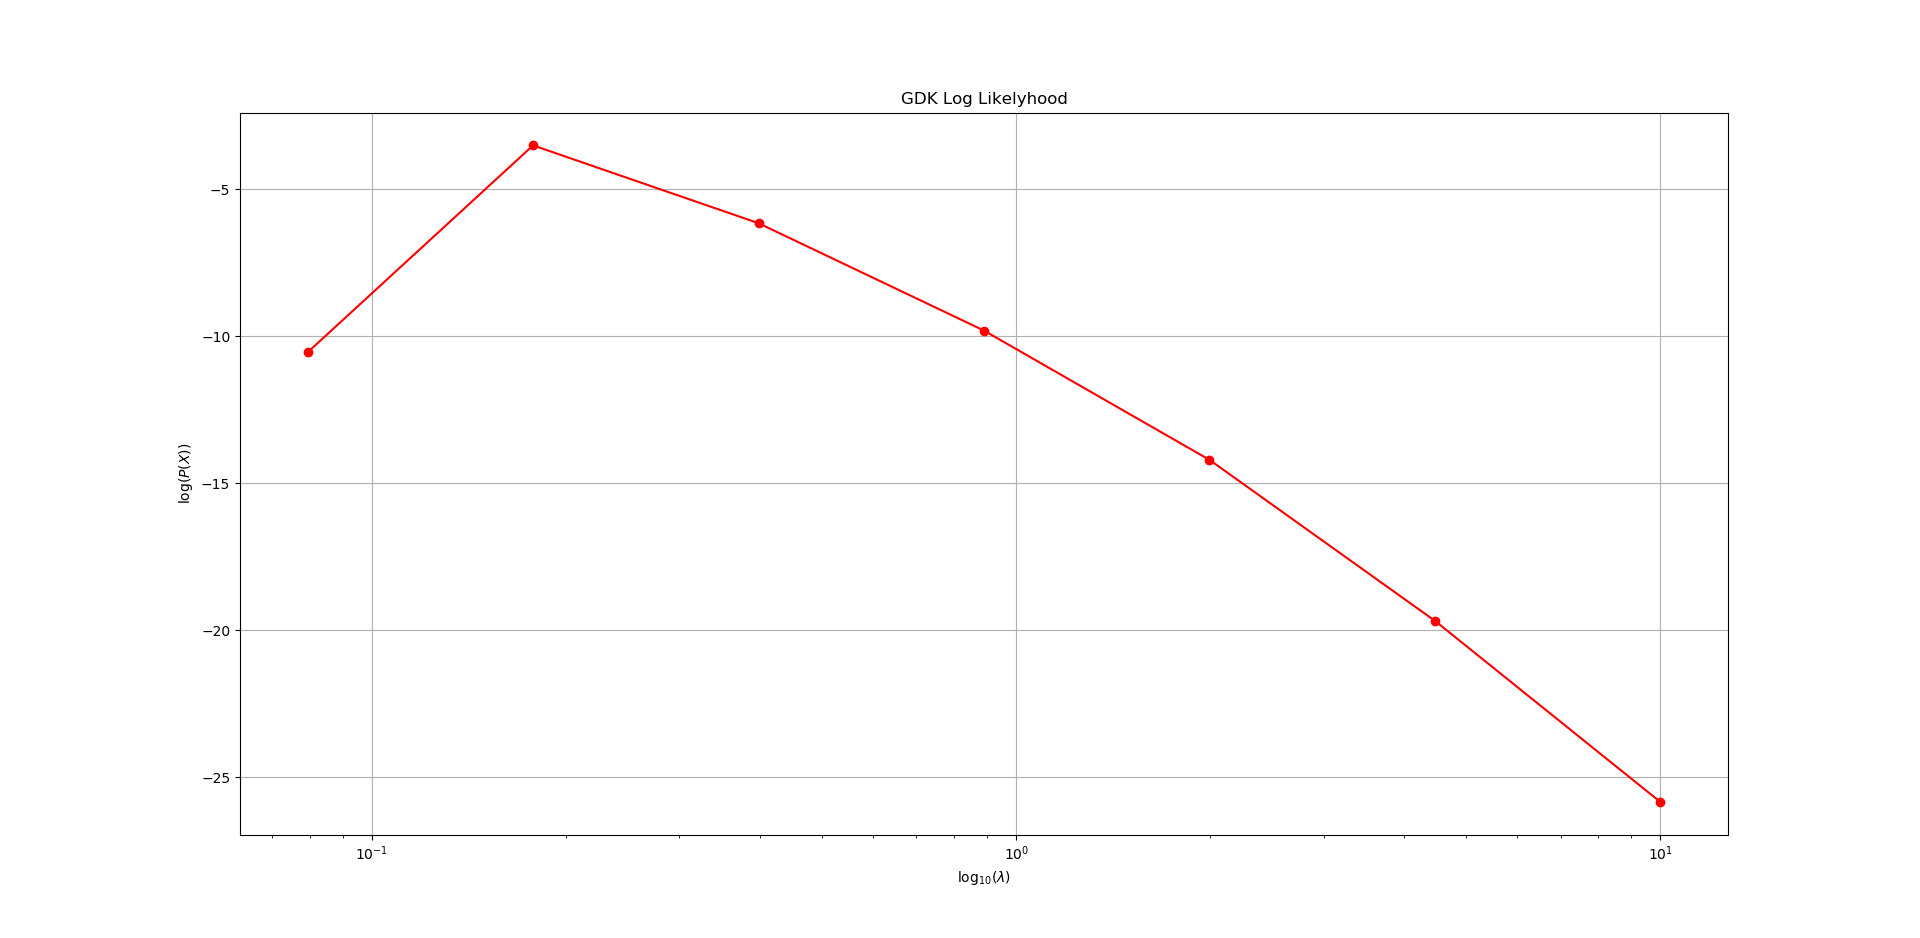
\includegraphics[width=.7\textwidth]{gdk}
	\caption{Mean log probabilities for different values of $ \lambda $.}
	\label{fig:lambdas}
\end{figure}\noindent

\paragraph{KNN Density (KNNDE)}
This method looks at the $ K $ nearest neighbours to a given observation and determines the density this way. We selected $ K=10 $ based on preliminary testing.
The density is then calculated as
\begin{equation*}
	\operatorname{density}_{\mathbf X}(x, K)=\frac{K}{\sum_{x'\in N_{x, K}}d(x, x')}, \quad d=\len{x-x'}
\end{equation*}
This method works well in many cases, but it has one major drawback, which the next method aims to solve.

\paragraph{KNN Average Relative Density (ARD)}
This method takes into account clusters of different densities such that dense clusters do not dominate as much, which is a major improvement over GDK and KNNDE.
It is build on KNNDE and calculated as
\begin{equation*}
	\operatorname{ard}_{\mathbf X}(x, K)=\frac{K\operatorname{density}_{\mathbf X}(x, K)}{\sum_{x_j \in N_{\mathbf X}}(x, K)\operatorname{density}_{\mathbf X_{\backslash j}}(x_j, K)}
\end{equation*}
Again, we used $ K=10 $.

\paragraph{Comparison}
We ranked all observations according to the different methods described. The results are shown on figure \eqref{fig:ting}.
\begin{figure}[H]
	\centering
	\begin{minipage}[t]{.3\textwidth}
		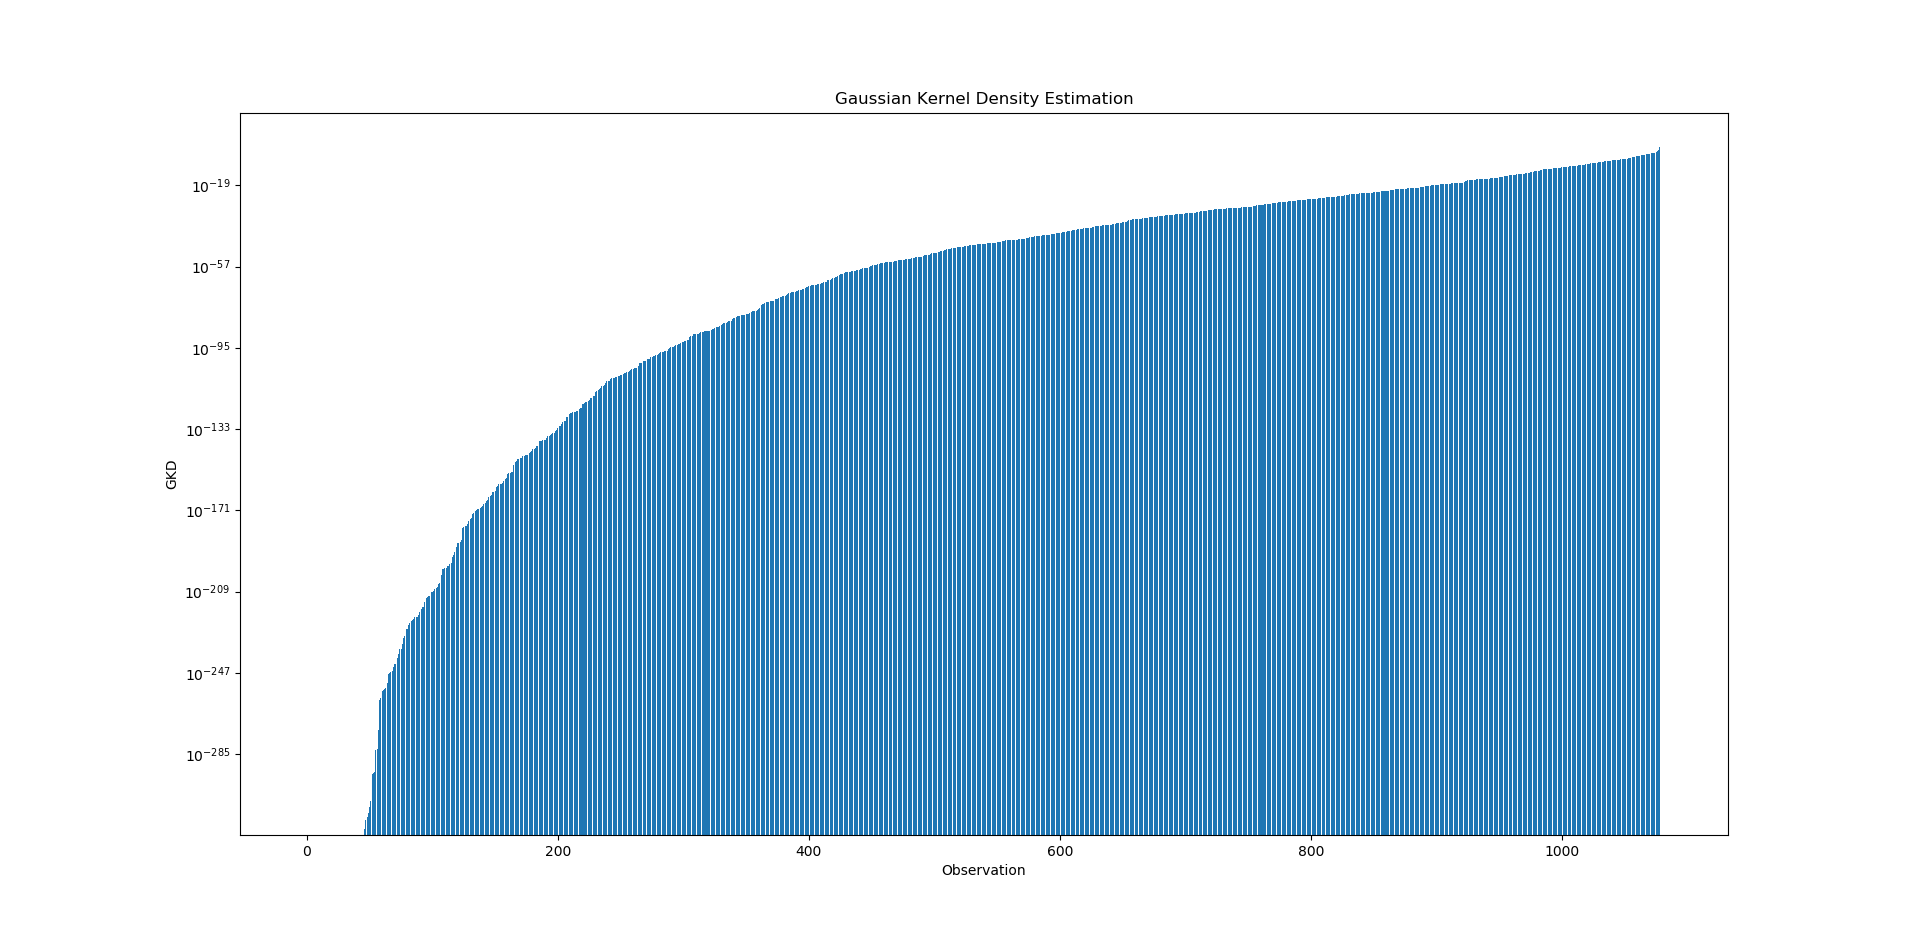
\includegraphics[width=\textwidth]{gdk-ll}
	\end{minipage}\hfill
	\begin{minipage}[t]{.3\textwidth}
		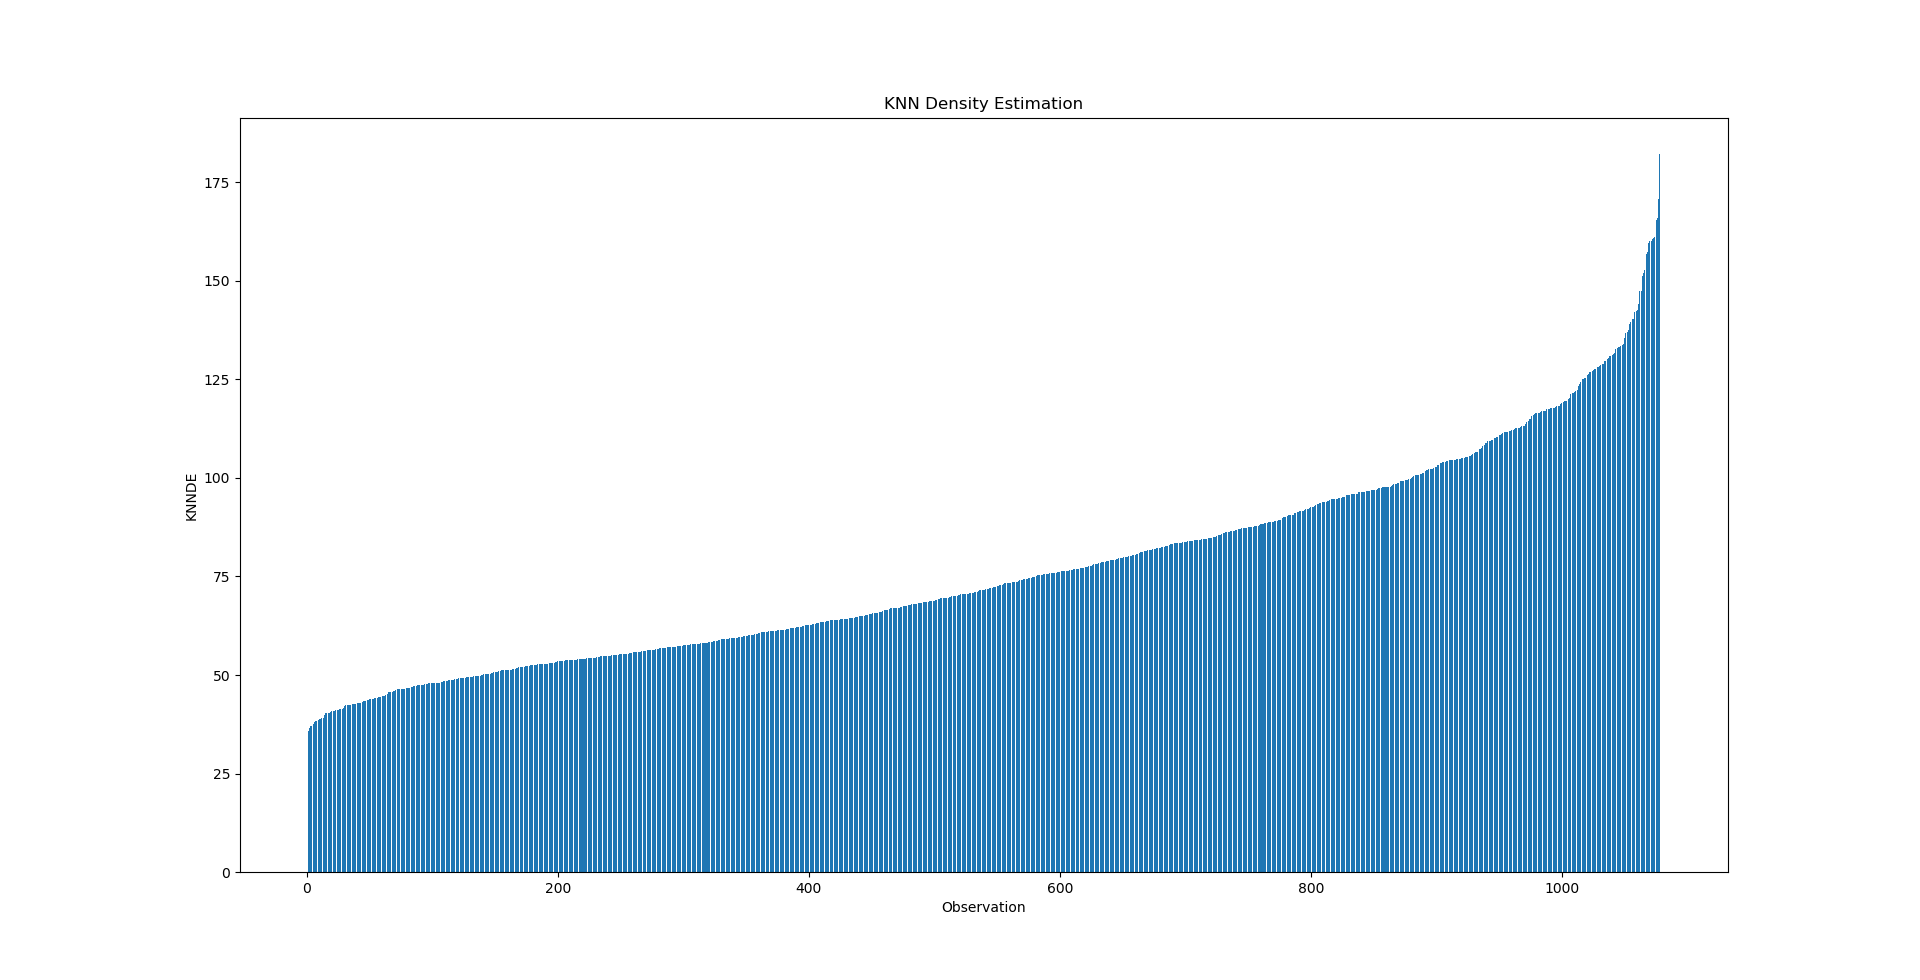
\includegraphics[width=\textwidth]{kde}
	\end{minipage}\hfill
	\begin{minipage}[t]{.3\textwidth}
		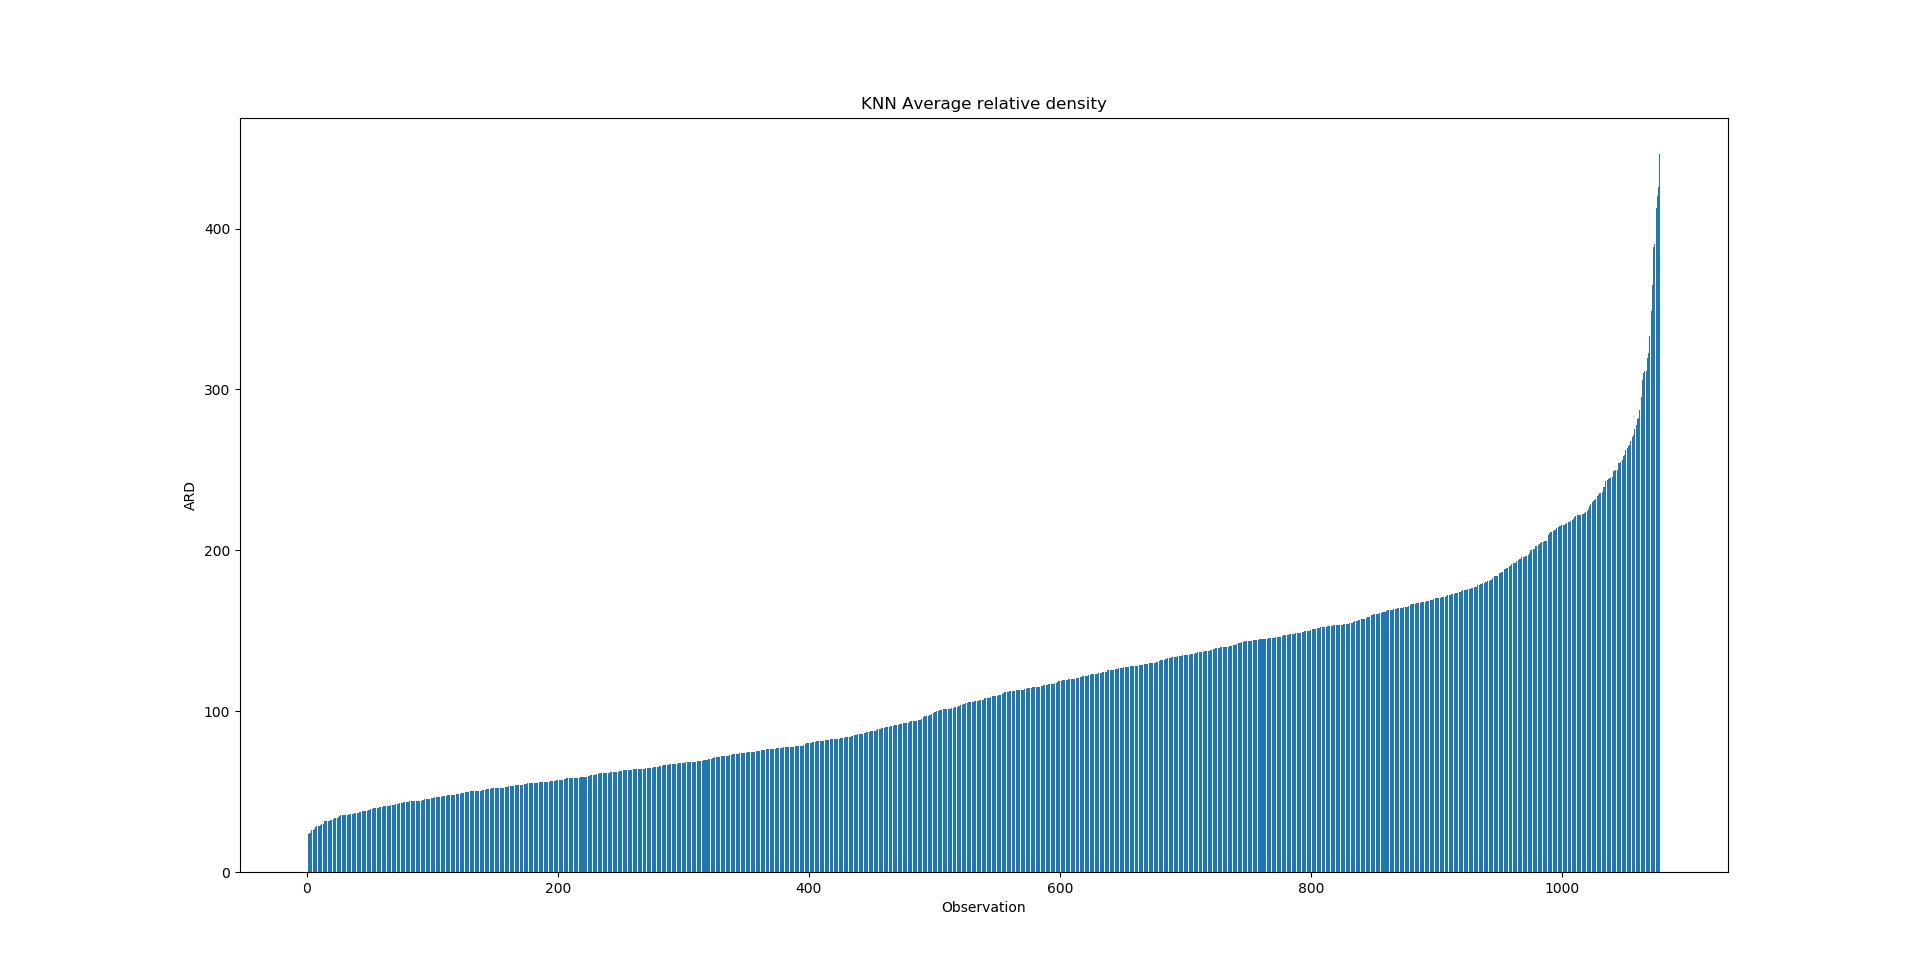
\includegraphics[width=\textwidth]{ard}
	\end{minipage}\hfill
	\caption{Outlier scoring with different methods.}\label{fig:ting}
\end{figure}\noindent
We opted to use a log scale for GKD as the values varied greatly.
GKD disagrees quite a bit with the remaining models, as it predicts a good chunk of the dataset to be outliers, whereas the other two methods show no clear outliers.














